\documentclass[12pt]{article}
\pagestyle{empty}
\usepackage{amsmath, amssymb, amsthm}
\usepackage{latexsym, epsfig, ulem, cancel, multicol, hyperref}
\usepackage{graphicx, tikz, subfigure,pgfplots}
\usepackage[margin=1in]{geometry}
\setlength{\parindent}{0pt}
\usepackage{multirow}
\usepackage{mathtools}
\usepackage{verbatim}
\usepackage{tikz}
\usepackage{pgfplots}
\setlength{\parskip}{1ex}

\newcommand{\T}[0]{\top}
\newcommand{\F}[0]{\bot}
\newcommand{\liminfty}[1]{\lim_{#1 \to \infty}}
\newcommand{\limzero}[1]{\lim_{#1 \to 0}}
\newcommand{\limto}[1]{\lim_{#1}}
\newcommand{\Z}{\mathbb{Z}}
\newcommand{\R}{\mathbb{R}}
\newcommand{\C}{\mathbb{C}}
\newcommand{\Q}{\mathbb{Q}}
\newcommand{\odd}[0]{\mathbb{Z} - 2\mathbb{Z}}
\newcommand{\lineint}[1]{\int_{#1}}
\newcommand{\pypx}[2]{\frac{\partial #1}{\partial #2}}
\newcommand{\divg}{\nabla \cdot}
\newcommand{\curl}{\nabla \times}
\newcommand{\dydx}[2]{\frac{d #1}{d #2}}
\newcommand{\sqbkt}[1]{\left[ #1 \right]}
\newcommand{\paren}[1]{\left( #1 \right)}
\newcommand{\tribkt}[1]{\left< #1 \right>}
\newcommand{\abso}[1]{\left|#1 \right|}
\newcommand{\zero}{\{0\}}
\newcommand{\then}{\rightarrow}
\newcommand{\nonneg}{\Z^+ \cup \{0\}}
\DeclarePairedDelimiter\ceil{\lceil}{\rceil}
\DeclarePairedDelimiter\floor{\lfloor}{\rfloor}
\newcommand{\union}[2]{\bigcup_{#1}^{#2}}
\newcommand{\inter}[2]{\bigcap_{#1}^{#2}}
\newcommand{\openclose}[1]{\left( #1 \right]}
\newcommand{\closeopen}[1]{\left[ #1 \right)}
\newcommand{\compo}[2]{#1 e^{i #2}}
\newcommand{\laplase}{\bigtriangleup}
\newcommand{\bra}[1]{\left< #1 \right|}
\newcommand{\ket}[1]{\left| #1 \right>}
\newcommand{\braket}[2]{\left< #1 \mid #2 \right>}
\newcommand{\ketbra}[2]{\left| #1 \right> \left< #2 \right|}
\newcommand{\ketpsit}{\ket{\psi(t)}}
\newcommand{\ketphit}{\ket{\phi(t)}}
\newcommand{\ham}{\mathbf{H}}
\newcommand{\unx}{\hat{\mathbf{x}}}
\newcommand{\uny}{\hat{\mathbf{y}}}
\newcommand{\unz}{\hat{\mathbf{z}}}
\newcommand{\uni}{\hat{\mathbf{i}}}
\newcommand{\unj}{\hat{\mathbf{j}}}
\newcommand{\unk}{\hat{\mathbf{k}}}
\newcommand{\uns}{\hat{\mathbf{s}}}
\newcommand{\unr}{\hat{\mathbf{r}}}
\newcommand{\untheta}{\hat{\boldsymbol\theta}}
\newcommand{\unphi}{\hat{\boldsymbol\phi}}
\newcommand{\unrho}{\hat{\boldsymbol\rho}}


\newcommand{\wsnumber}{1}
\newcommand{\wstopic}{Vectors}
\pgfplotsset{
    every linear axis/.append style={
       axis x line=center,
       axis y line=center,
       xlabel={$x$},
       ylabel={$y$}
    },
    every axis plot/.append style={thick,mark=none}
}
\tikzset{
    point/.style={circle,draw,fill,minimum width=0.3ex,inner sep=0pt,outer sep=0pt},
    every label/.append style={black}
}


\usepackage[margin=1in]{geometry}
\usepackage{amsmath, amssymb, amsthm, graphicx, hyperref}
\usepackage{enumerate}
\usepackage{fancyhdr}
\usepackage{multirow, multicol}
\usepackage{tikz}
\pagestyle{fancy}
\fancyhead[RO]{Dennis Li}
\fancyhead[LO]{Analytical Mechanics }
\usepackage{comment}
\newif\ifshow
\showfalse

\ifshow
  \newenvironment{solution}{\textbf{Solution.}}{}
\else
  \excludecomment{solution}
\fi

\renewcommand{\thefootnote}{\fnsymbol{footnote}}
\usepackage{comment}


\newtheorem*{remark}{Remark}


\begin{document}
\begin{center}
\ifshow
  \textbf{\Large Problem Set 01 Solution}\\
\else
  \textbf{\Large Problem Set 01}\\
\fi
Instructor \\ Prof. Gabe\\
\end{center}

\hrule

\vspace{0.2cm}



\begin{enumerate}
    \item[MT5 1.9] For these two vectors
\[
\mathbf{A} = \hat{i} + 2\hat{j} - \hat{k}, \quad \mathbf{B} = -2\hat{i} + 3\hat{j} + \hat{k}
\]
find
\begin{enumerate}
    \item \(\mathbf{A} - \mathbf{B}\) and \(|\mathbf{A} - \mathbf{B}|\)
    \[
    \mathbf{A} - \mathbf{B} = (1+2)\uni + (2-3)\unj + (-1-1)\unk = 3\uni - \unj - 2\unk
    \]
    \[
    \abso{-\uni + 5 \unj} = \sqrt{1+5^2} = \sqrt{26}
    \]
    \item component of \(\mathbf{B}\) along \(\mathbf{A}\).
    
    This can be found by projecting \textbf{B} onto \textbf{A}. Let \textbf{C} be the component of \textbf{B} along \textbf{A}. Let $\hat{\mathbf{A}}$ be the \textit{unit vector} of \textbf{A}.
    \[
    \mathbf{C} = \frac{\mathbf{A}\cdot \mathbf{B}}{\abso{\mathbf{A}}} = \frac{-2+6-1}{\sqrt{1+4+1}} = \frac{3}{\sqrt{6}}\hat{\mathbf{A}}
    \]
    
    \item angle between \(\mathbf{A}\) and \(\mathbf{B}\)
    By definition of the dot product, we have
    \[
    \mathbf{A}\cdot \mathbf{B} = \abso{\mathbf{A}}\abso{\mathbf{B}}\cos\phi
    \]
    Therefore
    \[
    \phi = \cos^{-1}\paren{\frac{\mathbf{A}\cdot \mathbf{B}}{\abso{\mathbf{A}}\abso{\mathbf{B}}}} = \cos^{-1}\paren{\frac{3}{\sqrt{6}\cdot \sqrt{15}}} = \cos^{-1}\paren{\frac{1}{\sqrt{10}}} \approx 1.249 \; \text{rad}
    \]
    Or $\phi = 71.56^\circ$.
    
    \item \(\mathbf{A} \times \mathbf{B}\)
    We can calculate this with the determinant of the following matrix
    \[
    \abso{
    \begin{matrix}
        \uni & \unj & \unk\\
        1 & 2 & -1\\
        -2& 3 & 1
    \end{matrix}
    } = 5\uni + \unj + 7\unk 
    \]
    
    
    \item \((\mathbf{A} - \mathbf{B}) \times (\mathbf{A} + \mathbf{B})\)
    We find the sum and differences of \textbf{A} and \textbf{B} first.
    \[
    \mathbf{A} + \mathbf{B} = 3\uni + \unj - 2\unk
    \]
    \[
    \mathbf{A} - \mathbf{B} = -\uni + 5\unj 
    \]
    Now we do the same thing as before
    \[
    \abso{
    \begin{matrix}
        \uni & \unj & \unk\\
        3 & -1 & -2\\
        -1& 5 & 0
    \end{matrix}
    } = 7\uni -2\unj + 14\unk 
    \]
\end{enumerate}

    \item[T1 1.5]Find the angle between a body diagonal of a cube and any one of its face diagonals. \textit{[Hint: Choose a cube with side 1 and with one corner at $O$ and the opposite corner at the point $(1, 1, 1)$. Write down the vector that represents a body diagonal and another that represents a face diagonal, and then find the angle between them as in Problem 1.4.]}

    To solve this, we first define a cube that situates in the first octant, and one of the corner at $(0,0,0)$, and the opposite corner at $1,1,1$. And the body diagonal can be characterized as a vector pointing from $(0,0,0)$ to $(1,1,1)$. We define this by $\mathbf{a} = \tribkt{1,1,1}$. And we can define one of the face vector t0 be going from $(0,0,0)$ to $(1,1,0)$, and written as $\mathbf{b} = \tribkt{1,1,0}$

    Now, we can calculate the angle between them with the definition of a dot product just like we did before.
    \[
    \phi = \cos^{-1}\paren{\frac{\mathbf{a}\cdot\mathbf{b}}{\abso{\mathbf{a}}\abso{\mathbf{b}}}} = \cos^{-1}\paren{\frac{2}{\sqrt{2}\sqrt{6}}} \simeq 0.6155
    \]
    Or $\phi \simeq 35.26^\circ$

    \item[T1 1.6] By evaluating their dot product, find the values of the scalar $s$ for which the two vectors
        \[
        \mathbf{b} = \unx + s\uny \quad \text{and} \quad \mathbf{c} = \unx - s\uny
        \]
        are orthogonal. (Remember that two vectors are orthogonal if and only if their dot product is zero.) Explain your answers with a sketch.

        If we want the vectors to be orthogonal, or $\mathbf{b}\perp \mathbf{c}$, we know that $\mathbf{b}\cdot \mathbf{c} = 0$. Now we can expand their dot product and get
        \[
        \textbf{b} \cdot \textbf{c} = 1 -s^2 = 0
        \]
        Therefore we have the equation
        \[
        s^2 = 1
        \]
        And $s = \pm1$ is the solution to this equation. We can plot these 2 vectors and they look like follows, see \textit{Figure} \ref{fig:1.6}
        \begin{figure}[!h]
            \centering
            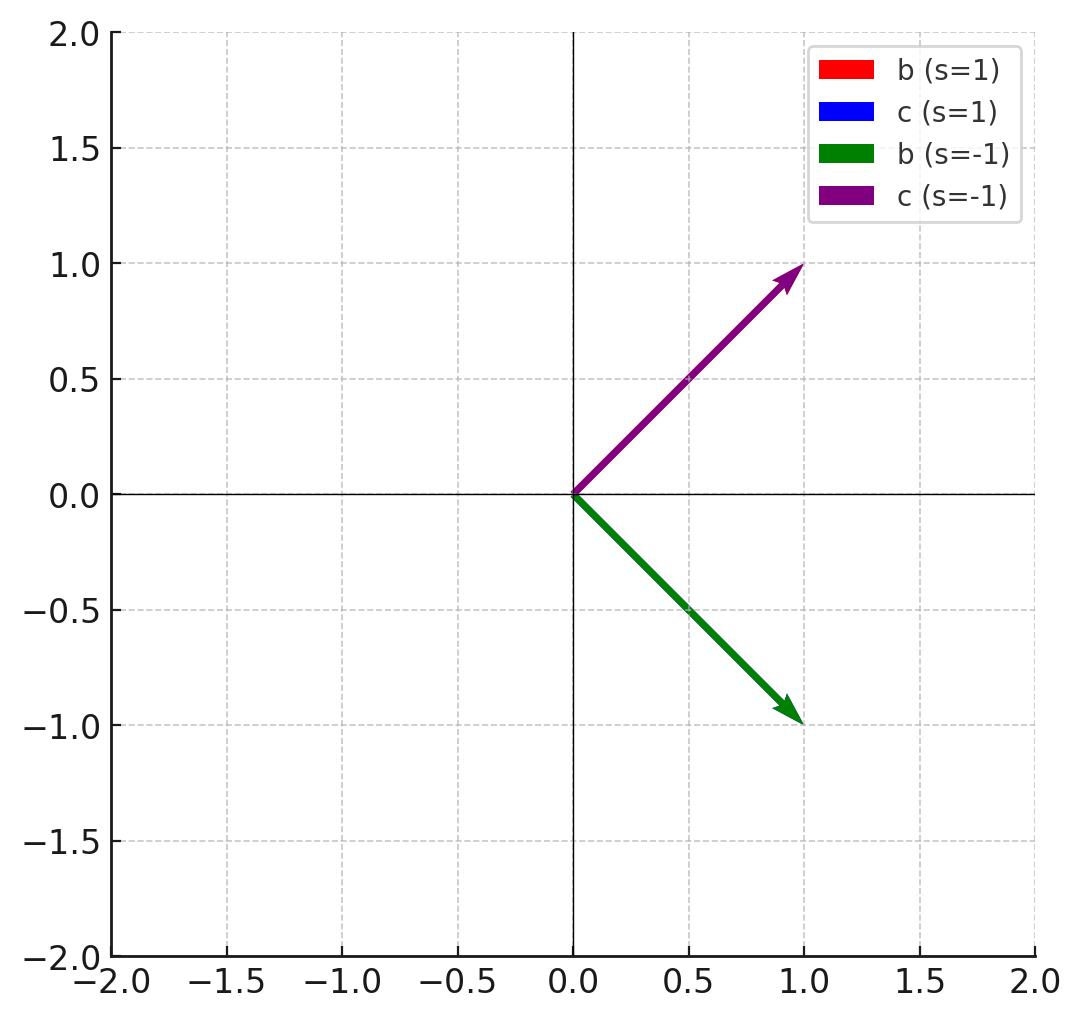
\includegraphics[width=0.3\linewidth]{Pictures/PS00/T1-1-6.png}
            \caption{Picture for T1 1.6}
            \label{fig:1.6}
        \end{figure}
        We can interpret $\mathbf{b}$ and $\mathbf{c}$ as a reflection about the $x$ axis. Since the $\unx$ component of the vector is fixed, we essentially have to find a line that is perpendicular to its reflection about the $x$ axis. And this leaves us to only 2 choices. So $\mathbf{b}$ has to be $\unx + \uny$ or $\unx - \uny$ while $\mathbf{c}$ be the other one. 
        
    \item[T1 1.9] In elementary trigonometry, you probably learned the law of cosines for a triangle of sides $a$, $b$, and $c$, that 
        \[
        c^2 = a^2 + b^2 - 2ab \cos \theta
        \]
        where $\theta$ is the angle between the sides $a$ and $b$. Show that the law of cosines is an immediate consequence of the identity 
        \[
        (\mathbf{a} + \mathbf{b})^2 = \mathbf{a}^2 + \mathbf{b}^2 + 2\mathbf{a} \cdot \mathbf{b}.
        \]

        \begin{proof}
            First we define $\mathbf{a}$ and $\mathbf{b}$ to be two vectors. And we should rewrite the identity since $(\mathbf{a} + \mathbf{b})^2, \mathbf{a}^2, \mathbf{b}^2$ are poorly defined. We are actually working with
            \[
            \paren{\mathbf{a}+\mathbf{b}}\cdot \paren{\mathbf{a}+\mathbf{b}} = \abso{\mathbf{a}}^2 + \abso{\mathbf{b}}^2 + 2\mathbf{a}\cdot \mathbf{b}
            \]
            We define the magnitude of the vector to be the side of the triangle, therefore 
            \[
            a = \abso{\mathbf{a}} \quad b = \abso{\mathbf{b}}
            \]
            And we define the sum of the vector to be
            \[
            \mathbf{c} = \mathbf{a}+\mathbf{b}
            \]
            By the essence of vector addition, the vector $\mathbf{c}$ will be the third side of the triangle. And we know that $\mathbf{c}\cdot \mathbf{c} = \abso{\mathbf{c}}^2$. We define $c = \abso{\mathbf{c}}$. Now we have the simplified expression.
            \[
            c^2 = a^2 + b^2 + 2\mathbf{a}\cdot\mathbf{b}
            \]
            By definition of dot product, we can expand it to 
            \[
            c^2 = a^2 + b^2 + 2ab\cos\phi
            \]
            The problem with this result is that, $\phi$ is the angle between the 2 vectors when they are connected \textit{tail to tail}. But the triangle they form would require us to connect them \textit{tip to tail}, and that provides a very different angle. If we would look at a generic example with 2 arbitrary vector, we can see that the actual angle we are working with is $\theta = \pi - \phi$. Details can be seen in \textit{Figure} \ref{fig:1.9} If we would plug it into a cosine, since cosine is even, this becomes
            \[
            c^2 = a^2 + b^2 + 2ab\cos\paren{\phi - \pi}
            \]
            This is effectively changing the phase of cosine by exactly $-\pi$. And we know that $\cos(\phi - \pi) = -\cos\phi$. Therefore we have arrived at
            \[
            c^2 = a^2 + b^2 - 2ab\cos\phi
            \]
            \begin{figure}
                \centering
                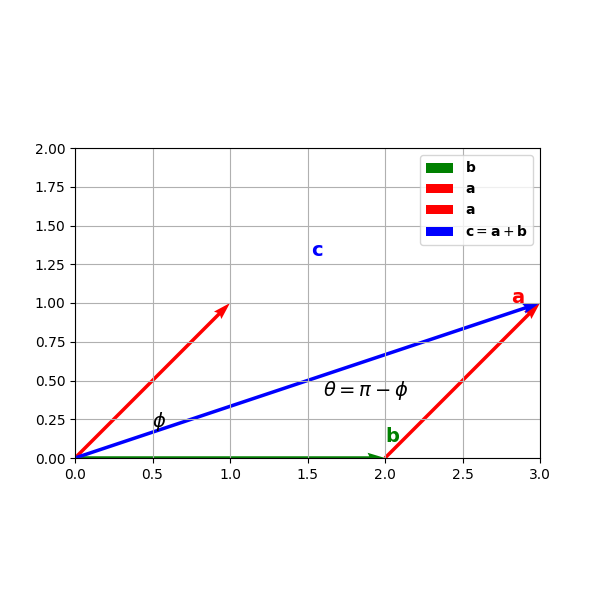
\includegraphics[width=0.4\linewidth]{Pictures/PS00/Figure_2.png}
                \caption{$\phi$ and $\theta$}
                \label{fig:1.9}
            \end{figure}
        \end{proof}

    \item[T1 1.10] A particle moves in a circle (center $O$ and radius $R$) with constant angular velocity $\omega$ counterclockwise. The circle lies in the $xy$ plane and the particle is on the $x$ axis at time $t = 0$. Show that the particle's position is given by
        \[
        \mathbf{r}(t) = s \cos(\omega t)\unx +  s \sin(\omega t)\uny
        \]
        Find the particle's velocity and acceleration. What are the magnitude and direction of the acceleration? Relate your results to well-known properties of uniform circular motion. 
        
        We would use \textit{Figure} \ref{fig:1.10}
            \begin{figure}[!h]
                \centering
                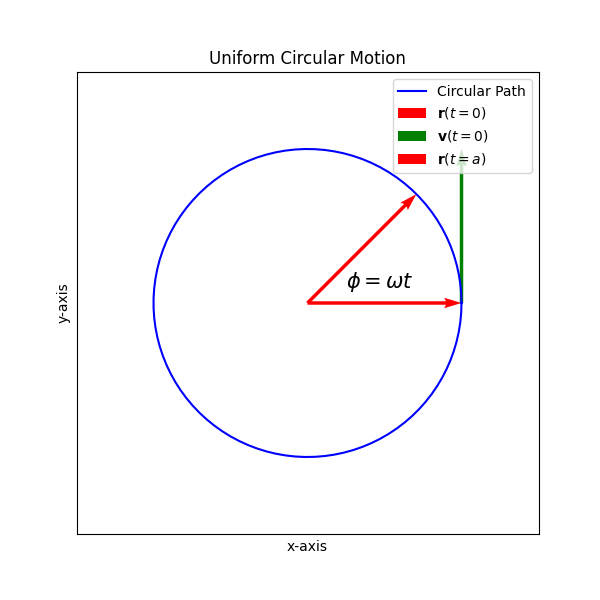
\includegraphics[width=0.4\linewidth]{Pictures/PS00/Figure_3c.png}
                \caption{Visualization of such motion}
                \label{fig:1.10}
            \end{figure}

        We see that the angle made between the position vector $\mathbf{r}$ and the horizontal axis is $\phi = \omega t$ as time progress. And we can obtain the $\unx$ and $\uny$ components using cosine and sine. This gives us 
        \[
        \mathbf{r}(t) = s \cos(\omega t)\unx +  s \sin(\omega t)\uny
        \]
        Where $s$ is the radius of the circular path, or in this case, the magnitude of $\mathbf{r}$. To find its velocity vector, we simply take the time derivative of the position vector. Since the radius $s$ and angular velocity $\omega$ are constants, we are only interested in $t$. 
        \[
        \mathbf{v}(t) = \dot{\mathbf{r}}(t) = -\omega s\sin(\omega t)\unx + \omega s\cos(\omega t)\uny
        \]
        To find the acceleration, we simply take another time derivative.
        \[
        \mathbf{a}(t) = \dot{\mathbf{v}}(t) = -\omega^2s\cos(\omega t) \unx - \omega^2 s\sin(\omega t)\uny
        \]
        We can do some factoring, and obtain
        \[
        \mathbf{a}(t) = -\omega^2 \mathbf{r}(t)
        \]
        The direction is opposite to the position vector as seen by the $-\omega^2$ multiplier before the positional vector. The magnitude of the acceleration can be defined as $a = \sqrt{\mathbf{a}\cdot \mathbf{a}}$. If we carry out this calculation.
        \[
        a = \sqrt{\paren{-\omega^2}\paren{-\omega^2}\paren{\mathbf{r}\cdot\mathbf{r}}}
        \]
        But we already know that the magnitude of the position vector is the radius of the circle, or $\mathbf{r}\cdot\mathbf{r}=\abso{\mathbf{r}}^2=s^2$. Therefore we can simplify it as follows
        \[
        a = \sqrt{\omega^4s^2} = \omega^2s
        \]
        Which perfectly aligns with our well-known definition of the centripetal acceleration formula $a_c = \omega^2 r$, where $r$ is the radius of the circular path. 

        \item[MT5 1.13] \textbf{X} is an unknown vector satisfying the following relations involving the known vectors \textbf{A} and \textbf{B} and the scalar \( \phi \),
        \[
        \mathbf{A} \times \mathbf{X} = \mathbf{B}, \quad \mathbf{A} \cdot \mathbf{X} = \phi.
        \]
        Express \textbf{X} in terms of \textbf{A}, \textbf{B}, \( \phi \), and the magnitude of \textbf{A}.

        We can first try to define the following cross product.
        \[
        \mathbf{C} = \mathbf{A}\times\paren{\mathbf{A}\times \mathbf{X}}
        \]
        We can manipulate this cross product with the BAC-CAB rule.
        \[
        \mathbf{A}\times\paren{\mathbf{A}\times \mathbf{X}} = \mathbf{A}\paren{\mathbf{A}\cdot\mathbf{X}} - \paren{\mathbf{A}\cdot\mathbf{A}}\mathbf{X}
        \]
        We can define $A = \abso{\mathbf{A}}$. And this can be then rewritten as
        \[
        \mathbf{A}\times\mathbf{B} = \phi\mathbf{A}- A\mathbf{X}
        \]
        By moving things around and cleaning up a little, we will finally obtain
        \[
        \mathbf{X} = \frac{-\mathbf{A}\times\mathbf{B} + \phi\mathbf{A}}{A}
        \]

        \item[MT5 1.24] Let \(\mathbf{A}\) be an arbitrary vector, and let \(\mathbf{e}\) be a unit vector in some fixed direction. Show that
        \[
        \mathbf{A} = \mathbf{e} (\mathbf{A} \cdot \mathbf{e}) + \mathbf{e} \times (\mathbf{A} \times \mathbf{e})
        \]
        What is the geometrical significance of each of the two terms of the expansion?

        \begin{proof}
            First, we can refine the notation a little. Since $\mathbf{e}$ is a unit vector, we can instead denote it as $\hat{\mathbf{e}}$. First of all, we should analyze
        \[
        \hat{\mathbf{e}}\paren{\mathbf{A}\cdot \hat{\mathbf{e}}}
        \]
        The dot product $\mathbf{A}\cdot \hat{\mathbf{e}}$ gives us the magnitude of the component of $\mathbf{A}$ on the $\hat{\mathbf{e}}$ direction. And if we scale $\hat{\mathbf{e}}$ with this component of $\mathbf{A}$ on $\hat{\mathbf{e}}$, we get the $\hat{\mathbf{e}}$ vector component of the vector $\mathbf{A}$, and that is $\paren{\mathbf{A}\cdot \hat{\mathbf{e}}}\hat{\mathbf{e}}$. Here, we denote it as $\mathbf{A}_\parallel = \hat{\mathbf{e}}\paren{\mathbf{A}\cdot \hat{\mathbf{e}}}$, or the parallel component of $\mathbf{A}$.

        Now, we examine the second term with the BAC-CAB rule.
        \[
        \hat{\mathbf{e}}\times \paren{\mathbf{A}\times\hat{\mathbf{e}}} = \mathbf{A}\paren{\hat{\mathbf{e}}\cdot\hat{\mathbf{e}}} - \hat{\mathbf{e}}\paren{\mathbf{A}\cdot\hat{\mathbf{e}}}
        \]
        Here, we notice that $\hat{\mathbf{e}}\cdot \hat{\mathbf{e}} = 1$ since it is a unit vector, and the second term is $\mathbf{A}_\parallel$ that we have just analyzed. Then the expression can be further simplified as
        \[
         \hat{\mathbf{e}}\times \paren{\mathbf{A}\times\hat{\mathbf{e}}} = \mathbf{A} - \mathbf{A}_\parallel
        \]
        We notice that $\mathbf{A} - \mathbf{A}_\parallel$ is precisely the vertical component of $\mathbf{A}$ with respect to the unit vector $\hat{\mathbf{e}}$. Therefore we can denote it as $\mathbf{A}_\perp = \mathbf{A} - \mathbf{A}_\parallel$. And once we realize this relationship, we can very naturally see the connection below
        \[
        \mathbf{A} = \mathbf{A}_\perp + \mathbf{A}_\parallel
        \]
        This connection is true. And if we are to substitute the vertical and the parallel component to the expression they represents, we have shown that
        \[
        \mathbf{A} = \mathbf{e} (\mathbf{A} \cdot \mathbf{e}) + \mathbf{e} \times (\mathbf{A} \times \mathbf{e})
        \]
        \end{proof}
        \newpage
        Geometrically, we can think of $\mathbf{A}_\perp$ and $\mathbf{A}_\parallel$ as 2 sides of a right triangle where the side $\mathbf{A}_\parallel$ is co-linear with the unit vector $\hat{\mathbf{e}}$, and the vertical component $\mathbf{A}_\perp$ makes up the other right side of the triangle. Then, the vector $\mathbf{A}$ will be our hypotenuse. Refer to \textit{Figure} \ref{fig:1.24}.
            \begin{figure}[!h]
                \centering
                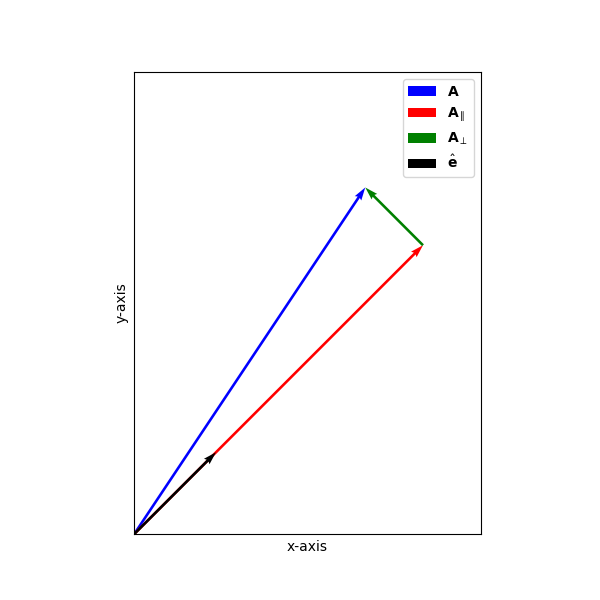
\includegraphics[width=0.5\linewidth]{Pictures/PS00/Figure_4.png}
                \caption{Geometrical Representation}
                \label{fig:1.24}
            \end{figure}

    \item[T1 1.13]Let $\mathbf{u}$ be an arbitrary fixed unit vector and show that any vector $\mathbf{b}$ satisfies
        \[
        b^2 = (\mathbf{u} \cdot \mathbf{b})^2 + (\mathbf{u} \times \mathbf{b})^2
        \]
        Explain this result in words, with the help of a picture.

        First of all, we have to specify what each term means. The left hand side would simply mean the magnitude of $\mathbf{b}$, therefore
        \[
        b^2 = \abso{\mathbf{b}}^2
        \]
        And the first term of the left hand side is the square of the dot product that is a scalar. The second term would define the square of the magnitude of the vector created by the cross product. 

        After clearing up what the notations mean, we can proceed to show that this relationship stands.
        \begin{proof}
            We start by using 
            First we can use the definition to manipulate the 2 terms involved
            \[
            \begin{cases}
                \abso{\mathbf{u}\cdot\mathbf{b}} = ub\cos\phi = b\cos\phi\\
                \abso{\mathbf{u}\times\mathbf{b}} = ub\sin\phi =b\sin\phi
            \end{cases}
            \]
            We define $u = \abso{\mathbf{u}}$ and $b = \abso{\mathbf{b}}$ Since \textbf{u} is a unit vector, it's magnitude is simply $1$, and $\phi$ is the angle between the two vectors. Now, we can find the product of their square
            \[
            (\mathbf{u} \cdot \mathbf{b})^2 + (\mathbf{u} \times \mathbf{b})^2 = \abso{\mathbf{u}\cdot\mathbf{b}}^2 + \abso{\mathbf{u}\times\mathbf{b}}^2
            \]
            Now we can substitute our results in
            \begin{align*}
               &\abso{\mathbf{u}\cdot\mathbf{b}}^2 + \abso{\mathbf{u}\times\mathbf{b}}^2\\
               &= \paren{b\cos\phi}^2 + \paren{b\sin\phi}\\
               &= b^2 \paren{\cos^2\phi + \sin^2\phi}\\
               &=b^2
            \end{align*} 
        \end{proof}
        What happened here is very similar to our previous question \textit{MT5 1.24}. The dot products produced a vector parallel to the unit vector $\mathbf{u}$. And the cross product created a vector that is orthogonal to both $\mathbf{b}$ and $\mathbf{u}$, and it's magnitude happen to be the same as if we would subtract the vectors as $\mathbf{b} - \mathbf{b}_\parallel$. Since they form a right triangle, the squared sum of the magnitude of the 2 orthogonal vectors will equal to the hypotenuse, and this become something analogous to the Pythagoras theorem. 

        \item[MT5 1.31] Show that
        \begin{enumerate}[(a)]
            \item \(\nabla r^n = nr^{n-2}\mathbf{r}\)

            \begin{proof} Define $\mathbf{r}\coloneqq \tribkt{x,y,z}$, then $r = \abso{\mathbf{r}} = \sqrt{x^2 + y^2 + z^2}$. We start by evaluating the gradient.
                \[
                \nabla r^n = \tribkt{\pypx{}{x}r^n, \pypx{}{y}r^n, \pypx{}{z}r^n}
                \]
                We can evaluate the first term in the gradient vector as an example 
                \[
                \pypx{}{x}\paren{\sqrt{x^2 + y^2 + z^2} }^n= \frac{nx}{\sqrt{x^2 + y^2 + z^2}}\paren{\sqrt{x^2 + y^2 + z^2} }^{n-1}
                \]
                We can keep simplifying the expression
                \begin{align*}
                &\frac{nx}{\sqrt{x^2 + y^2 + z^2}}\paren{\sqrt{x^2 + y^2 + z^2} }^{n-1} \\
                &= \frac{nx}{r}r^{n-1}\\
                &= nxr^{n-2}\\
                \end{align*}
                Repeat the process for all three components, and we get
                \[
                 \nabla r^n = \tribkt{nxr^{n-2},nyr^{n-2},nzr^{n-2}} = nr^{n-2}\tribkt{x,y,z}
                \]
                Since $\mathbf{r} = \tribkt{x,y,z}$, we have
                \[
                \nabla r^n = nr^{n-2}\mathbf{r}
                \]
            \end{proof}
            
            \item \( \nabla f(r) = \frac{\mathbf{r}}{r}\dydx{f}{r} \)

            \begin{proof}
                Define $\mathbf{r}\coloneqq \tribkt{x,y,z}$, then $r = \abso{\mathbf{r}} = \sqrt{x^2 + y^2 + z^2}$. Let $f(r)$ be a function of $r$. And if we take its gradient, we have
                \[
                \nabla f(r) = \tribkt{\pypx{}{x}f(r), \pypx{}{y}f(r),\pypx{}{z}f(r)}
                \]
                Now we can look at the partial derivative with respect to $x$ first.
                \[
                \pypx{}{x}f(r) = \pypx{r}{x}\dydx{f}{r} =\frac{x}{\sqrt{x^2 + y^2 + z^2}}\dydx{f}{r} = \frac{x}{r}\dydx{f}{r}
                \]
                We can obtain $\partial_y$ and $\partial_z$ similarly, the final gradient vector looks like
                \[
                \nabla f(r) = \tribkt{\frac{x}{r}\dydx{f}{r},\frac{y}{r}\dydx{f}{r},\frac{z}{r}\dydx{f}{r}}
                \]
                And if we would factor out $\frac{1}{r}\dydx{f}{r}$, since $\mathbf{r}=\tribkt{x,y,z}$, we have
                \[
                \nabla f(r) = \frac{\mathbf{r}}{r}\dydx{f}{r}
                \]
            \end{proof}
            \item \( \nabla^2\paren{\ln r} = \frac{1}{r^2} \)

            \begin{proof}
                Define $\mathbf{r}\coloneqq \tribkt{x,y,z}$, then $r = \abso{\mathbf{r}} = \sqrt{x^2 + y^2 + z^2}$. Now we can evaluate the gradient. Let $f(r) = \ln(r)$. We can use the result from the previous question to obtain
                \[
                \nabla\paren{\ln r} = \frac{\mathbf{r}}{r}\dydx{f}{r} = \frac{\mathbf{r}}{r^2}
                \]
                And now we take the divergence of the gradient vector to get the Laplacian.
                \[
                \divg\nabla\paren{\ln r} = \divg \frac{\mathbf{r}}{r^2}
                \]
                Now we can evaluate the divergence of $\frac{\mathbf{r}}{r^2}$
                \[
                \divg \frac{\mathbf{r}}{r^2} = \pypx{}{x}\frac{x}{r^2} + \pypx{}{y}\frac{y}{r^2} + \pypx{}{z}\frac{z}{r^2}
                \]
                As usual, we only look at $\partial_x$ as everything else is the same. 
                \[
                \pypx{}{x}\frac{x}{r^2} = \pypx{}{x} \frac{x}{x^2 + y^2 + z^2} 
                \]
                By quotient rule, this derivative evaluates to
                \[
                \pypx{}{x} \frac{x}{x^2 + y^2 + z^2}  = \frac{\paren{x^2 + y^2 + z^2} - 2x^2}{\paren{x^2 + y^2 + z^2}^2} = \frac{\paren{-x^2 + y^2 + z^2}}{\paren{x^2 + y^2 + z^2}^2}
                \]
                Similarly, we can find the other 2 term
                \[
                \pypx{}{y}\frac{y}{r^2} = \frac{\paren{x^2 - y^2 + z^2}}{\paren{x^2 + y^2 + z^2}^2} \quad 
                \pypx{}{z}\frac{z}{r^2} = \frac{\paren{x^2 + y^2 - z^2}}{\paren{x^2 + y^2 + z^2}^2} 
                \]
                If we add all 3 together, we have obtained
                \begin{align*}
                \divg \frac{\mathbf{r}}{r^2} &= \frac{\paren{-x^2 + y^2 + z^2}}{\paren{x^2 + y^2 + z^2}^2}+ \frac{\paren{x^2 - y^2 + z^2}}{\paren{x^2 + y^2 + z^2}^2}+\frac{\paren{x^2 + y^2 - z^2}}{\paren{x^2 + y^2 + z^2}^2}\\
                &= \frac{x^2 + y^2 + z^2}{\paren{x^2 + y^2 + z^2}^2}\\
                & = \frac{1}{x^2 + y^2 + z^2}\\
                &= \frac{1}{r^2}
                \end{align*}
                Therefore we have showed that
                \[
                \nabla^2\paren{\ln r} = \frac{1}{r^2}
                \]
            \end{proof}
        \end{enumerate}

    \newpage
    \item[T1 1.47] Let the position of a point \( P \) in three dimensions be given by the vector \( \mathbf{r} = (x, y, z) \) in rectangular (or Cartesian) coordinates. The same position can be specified by \textit{cylindrical polar coordinates}, \( \rho, \phi, z \), which are defined as follows: Let \( P' \) denote the projection of \( P \) onto the \( xy \) plane; that is, \( P' \) has Cartesian coordinates \( (x, y, 0) \). Then \( \rho \) and \( \phi \) are defined as the two-dimensional polar coordinates of \( P' \) in the \( xy \) plane, while \( z \) is the third Cartesian coordinate, unchanged.

        \begin{itemize}
            \item[(a)] Make a sketch to illustrate the three cylindrical coordinates. Give expressions for \( \rho, \phi, z \) in terms of the Cartesian coordinates \( x, y, z \). Explain in words what \( \rho \) is (``\( \rho \) is the distance of \( P \) from \_\_\_\_\_\_''). There are many variants in notation. For instance, some people use \( r \) instead of \( \rho \). Explain why this use of \( r \) is unfortunate.

            First, we can start by visualizing the spherical coordinate as shown in \textit{Figure} \ref{fig:1.47}. 
            \begin{figure}[!h]
                \centering
                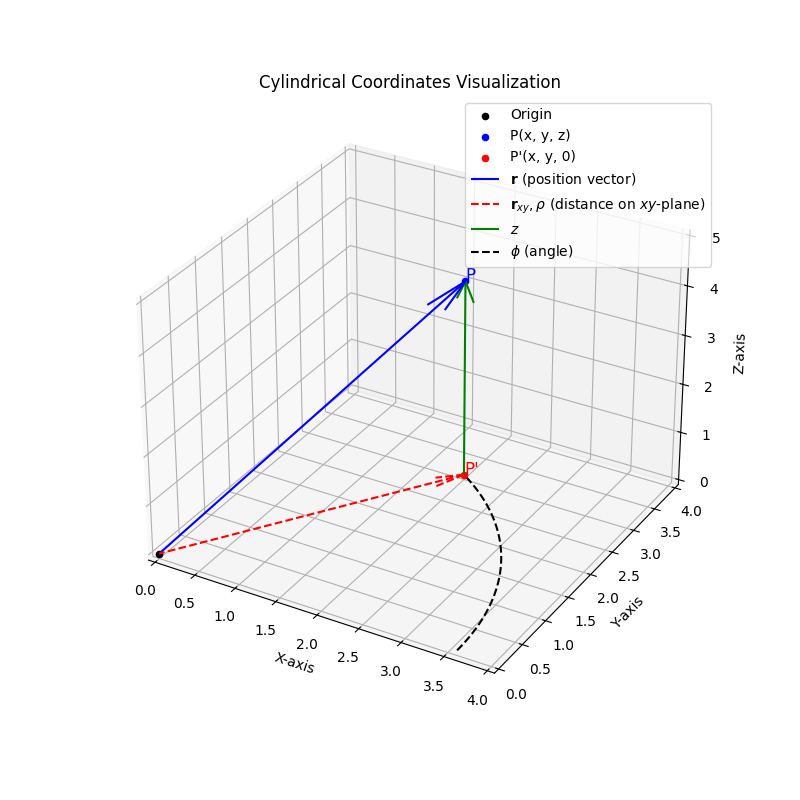
\includegraphics[width=0.5\linewidth]{Pictures/PS00/Figure_5.png}
                \caption{Cylindrical Coordinates}
                \label{fig:1.47}
            \end{figure}

            By examining the knowledge, we see that $z$ are not influenced when we change from Cartesian to Cylindrical. Therefore
            \[
            z=z
            \]
            Now we look at the projection onto $z=0$ plane. It is quite evident that this looks identical to what we have done in polar coordinates, since $z$ is not affected. We can write the remaining two components as
            \[
            \rho = \sqrt{x^2 + y^2} \quad \phi = \tan^{-1}\paren{\frac{y}{x}}
            \]
            Here, $\rho$ is the distance from the origin to the tip of the projection of $P$ on the $z=0$ plane, and $\rho$ is the angle it makes with the positive $x$ axis. 
            And by looking at \textit{Figure} \ref{fig:1.47}, we can see why the use of $r$ is not very useful here, since it does not really represent the \textit{radius} as we know it. It is simply the projection onto the $z=0$ plane. If we maintain using $r$, it will make things very hard to keep track. 
            
            \item[(b)] Describe the three unit vectors \( \unrho, \unphi, \unz \) and write the expansion of the position vector \( \mathbf{r} \) in terms of these unit vectors.

            With the knowledge from the image, we can derive the expression for $\unrho, \unphi, \unz$. We can tell from the image that $\boldsymbol{\rho}$ is the vector defined by $\mathbf{\rho} = x\unx + y\uny + 0\unz$ when the position vector $\mathbf{r} = x\unx + y\uny + z\unz$. This is fairly similar to the polar coordinate that we are familiar with since $\unz$ is in fact constant throughout the frame. Therefore we can simply write the unit vector $\unrho$ as 
            \[
            \unrho = \cos\phi \unx + \sin\phi \uny
            \]
            similarly to what we use to define $\unphi$ in 2D polar coordinate system, we can use the fact that $\unrho \cdot \unphi = 0$ to find that
            \[
            \unphi = -\sin\phi \unx + \cos\phi \uny
            \]
            Since the $z$ component is not changing in cylindrical coordinate, we do not need to work with transforming the $z$ coordinate. Therefore we have
            \[
            \unz = \unz
            \]
            And we can write our position vector as
            \[
            \mathbf{r} = \rho\unrho + z\unz
            \]
            Just like the polar coordinates, the position vector points radially outward and does not have a component of $\unphi$.
            
            \item[(c)] Differentiate your last answer twice to find the cylindrical components of the acceleration \( \mathbf{a} = \ddot{\mathbf{r}} \) of the particle. To do this, you will need to know the time derivatives of \( \unrho \) and \( \unphi \). You could get these from the corresponding two-dimensional results (1.42) and (1.46), or you could derive them directly as in Problem 1.48.

            Since $\unz$ is a constant, we only need to consider $z(t)$, $\rho(t)$, and $\unrho(t)$. Our first time derivative is
            \[
            \dot{\mathbf{r}} = \dot{\rho}\unrho + \rho\dot{\unrho} + \dot{z}\unz
            \]
            Let us examine the time derivative of $\rho$ and $\unrho$. Since they have the same expression as their $s$ and $\uns$ counterparts in 2D polar coordinates, we can simply use the result obtained from the derivation of the velocity vector in polar coordinates.
            \[
            \dot{\unrho} = -\Dot{\phi}\sin\phi\unx + \Dot{\phi}\cos\phi\uny = \Dot{\phi}\unphi
            \]
            And 
            \[
            \Dot{\unphi} = -\Dot{\phi}\cos\phi\unx - \Dot{\phi}\sin\phi\uny = - \Dot{\phi}\unrho
            \]
            The velocity vector can therefore be rewritten as
            \[
            \dot{\mathbf{r}} = \dot{\rho}\unrho + \rho\dot{\phi}\unphi + \dot{z}\unz
            \]
            And if we take the derivative again, we have
            \begin{align*}
                \dydx{}{t}\Dot{\mathbf{r}} &= \dydx{}{t}\paren{\Dot{\rho}\unrho + \rho\Dot{\phi}\unphi+\dot{z}\unz} \\
                \ddot{\mathbf{r}} &= \textbf{a} = \ddot{\rho}\unrho + \dot{\rho}\dot{\rho} + \dot{\rho}\Dot{\phi}\unphi + \rho\ddot{\phi}\unphi + \rho\dot{\phi}\dot{\unphi}+\ddot{z}\unz\\
                  \textbf{a}&= \ddot{\rho}\unrho + \dot{\rho}\dot{\phi}\unphi + \dot{\rho}\dot{\phi}\unphi + \rho\ddot{\phi}\unphi -  \rho\dot{\phi}^2\unrho+\ddot{z}\unz\\
                  \textbf{a}&= \paren{\ddot{\rho}-\rho\dot{\phi}^2}\unrho + \paren{2\dot{\rho}\dot{\phi}+\rho\ddot{\phi}}\unphi+\ddot{z}\unz
            \end{align*}


            
        \end{itemize}

    \newpage
    \item[MT5 1.25] Find the components of the acceleration vector \textbf{a} in spherical coordinates.

    To do this problem, we would first have to define our coordinate system in spherical coordinates. We can first look at a sketch of how it works in 3D Cartesian coordinates. Refer to \textit{Figure} \ref{fig:1.25}.
    \begin{figure}[!h]
        \centering
        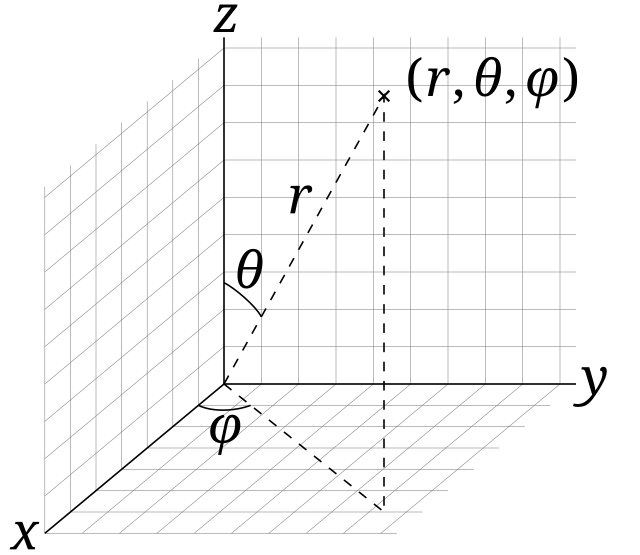
\includegraphics[width=0.5\linewidth]{Pictures/PS00/3D_Spherical.svg.png}
        \caption{Spherical Coordinates}
        \label{fig:1.25}
    \end{figure}
    To avoid confusion, we will use $\rho$ for radius instead of $r$, $r$ will be saved for the position vector. Let us define the \textit{'radius'} on the $z=0$ plane (like what we did in the previous question) as $\rho\sin\theta$. This gives us the distance from the origin to the tip of the projection on the $z=0$ plane. And from here, we can find the $x,y$ coordinates with angle $\phi$. Also, the $z$ coordinate is simply $\rho\cos\theta$ since this will land us on the $z$ axis. We now have the following relationship
    \[
    \begin{cases}
        x = \rho\sin\theta\cos\phi\\
        y = \rho\sin\theta\sin\phi\\
        z = \rho\cos\theta
    \end{cases}
    \]
    However, we are more interested in representing $\rho,\theta,\phi$ in terms of $x,y,z$. So we can define them as
    \[
    \begin{cases}
        \rho = \sqrt{x^2 + y^2 + z^2}\\
        \theta = \tan^{-1}\paren{\frac{\sqrt{x^2+y^2}}{z}}\\
        \phi = \tan^{-1}\paren{\frac{y}{x}}
    \end{cases}
    \]
    Now we have to find $\unrho,\unphi,\untheta$. The unit vector for $\rho$ is relatively easy, since it will be the normalized sum of $\unx,\uny,\unz$ components as it changes in space. So it can be defined as
    \[
    \unrho = \frac{1}{\rho}\paren{x\unx + y\uny + z\unz}
    \]
    We can use this information and plug in the expression for $x,y,z$ in spherical coordinates to get
    \[
    \unrho = \sin\theta\cos\phi \unx + \sin\theta\sin\phi\uny + \cos\theta \unz
    \]
    What we know about $\phi$ is that it should be orthogonal to $\unrho$ and $\untheta$. This means that $\unphi \cdot \unrho = 0$. And since it is on the $z=0$ plane, we can ignore the $\unz$ component in our expression for $\phi$. To make life easier, we define $\rho(z=0) = \varrho = \sqrt{x^2 + y^2}$. We can substitute $x$ and $y$ to obtain the polar expression for $\varrho$
    \[
    \varrho = \rho\sin\theta
    \]
    Now we can keep working on the expression
    \[
    \unrho(z=0) \cdot \unphi = \unrho = \frac{1}{\varrho}\paren{x\unx + y\uny} \cdot \paren{\phi_x\unx + \phi_y\uny} = 0
    \]
    This means that $x\phi_x + y\phi_y = 0$, or $x\phi_x = -y\phi_y$. This leaves only 1 possibly for solution
    \[
    \phi_x = -y \quad \phi_y = x
    \]
    And this gives us the expression for $\unphi$
    \[
    \unphi = \frac{-y\unx + x\uny}{\varrho} = \frac{-y\unx + x\uny}{\rho\sin\theta} 
    \]
    The $\varrho$ in the denominator normalizes the vector. We can substitute the expression for $x,y$ into this formula to get rid of them. In case of $\phi$, $z=0$ and $\theta = \frac{\pi}{2}$ since it is on the $z=0$ plane. This simplifies $\rho \to \varrho$. And the expression becomes something similar to its polar coordinate counterpart. 
    \[
    \unphi = -\sin\phi\unx + \cos\phi \uny
    \]
    After obtaining these 2 unit vectors, we can obtain $\untheta$ by the fact that $-\untheta = \unrho \times \unphi$. We can define this massive determinant
    \[
    -\untheta = \abso{
    \begin{matrix}
        \unx & \uny & \unz \\
        \frac{x}{\rho}&\frac{y}{\rho}&\frac{z}{\rho}\\
        \frac{-y}{\varrho}&\frac{x}{\varrho}&0
    \end{matrix}
    } = \frac{-xz}{\rho\varrho}\unx - \frac{yz}{\rho\varrho}\uny + \frac{x^2+y^2}{\rho\varrho}\unz
    \]
    After simplifying and substituting the expression for $\varrho$, we have
    \[
    \untheta = \frac{1}{\rho^2\sin\theta}\sqbkt{\paren{x\unx + y\uny}z - \paren{x^2+y^2}\unz}
    \]
    If we plug in the spherical coordinates expression for $x,y,z$, this simplifies to
    \[
    \untheta = \cos\theta\cos\phi \unx + \cos\theta\sin\phi \uny - \sin\theta \unz
    \]
    We have obtained the expression of unit vectors in spherical coordinates
    \[
    \begin{cases}
        \unrho = \sin\theta\cos\phi \unx + \sin\theta\sin\phi\uny + \cos\theta \unz\\
        \unphi = -\sin\phi\unx + \cos\phi \uny\\
        \untheta = \cos\theta\cos\phi \unx + \cos\theta\sin\phi \uny - \sin\theta \unz
    \end{cases}
    \]
    To obtain the expression for $\unx, \uny, \unz$ from this result, we need to know that $\unx$ has no $\uny,\unz$ components. So we can eximply extract the corresponding term from each unit vector and obtain
    \[
    \begin{cases}
        \unx = \sin\theta\cos\phi \unrho + \cos\theta\cos\phi \untheta -\sin\phi\unphi \\
        \uny = \sin\theta\sin\phi\unrho + \cos\theta\sin\phi\untheta +\cos\phi \unphi\\
        \unz =  \cos\theta\unrho - \sin\theta \untheta
    \end{cases}
    \]
    Now we can proceed to find the acceleration vector. Since the position vector points radially outward, we can easily define it in terms of spherical coordinate like what we did for polar. 
    \[
    \mathbf{r} = \rho\unrho
    \]
    We can take the time derivative of the position vector
    \[
    \dot{\mathbf{r}} = \dot{\rho}\unrho + \rho\dot{\unrho}
    \]
    Here, we have to find the time derivative of $\unrho,\unphi,\untheta$.
    \begin{align*}
        \dot{\unrho} &= \paren{\dot{\theta}\cos\theta\cos\phi -\dot{\phi}\sin\theta\sin\phi}\unx
                     + \paren{\dot{\theta}\cos\theta\sin\phi + \dot{\phi}\sin\theta\cos\phi}\uny
                     -\dot{\theta}\sin\theta \unz\\
                     &=\dot{\theta}\paren{\cos\theta\cos\phi \unx + \cos\theta\sin\phi \uny -\sin\theta\unz}+\dot{\phi}\sin\theta\paren{-\sin\phi \unx +\cos\phi \uny}\\
                     &= \dot{\theta}\untheta + \sin\theta\dot{\phi}\unphi
    \end{align*}
    \begin{align*}
        \dot{\untheta} &= -\paren{\dot{\theta}\sin\theta\cos\phi + \dot{\phi}\cos\theta\sin\phi}\unx + \paren{-\dot{\theta}\sin\theta\sin\phi + \dot{\phi}\cos\theta\cos\phi}\uny - \dot{\theta}\cos\theta\unz\\
                       &=-\dot{\theta}\paren{\sin\theta\cos\phi\unx + \sin\theta\sin\phi\uny +\cos\theta\unz} + \dot{\phi}\cos\theta\paren{-\sin\phi\unx + \cos\phi \uny}\\
                       &= -\dot{\theta}\unrho + \cos\theta\dot{\phi}\unphi
    \end{align*}
    \begin{align*}
        \dot{\unphi} &= -\dot\phi\cos\phi \unx - \dot\phi\sin\phi \uny\\
                    &= -\dot\phi\paren{\cos\phi \unx + \sin\phi \uny}\\
                    &= -\dot\phi\paren{\sin\theta\unrho + \cos\theta\untheta}
    \end{align*}
    Here, we notice that $\unrho$ points radially outward and $\untheta$ steers the radial vector away from $z$ axis. Therefore if we add these two unit vectors together, we get a vector pointing radially outward but only on the $z=0$ plane. We then scale them accordingly to make them unit vectors. 
    Now we can find the velocity vector
    \[
    \dot{\mathbf{r}} = \mathbf{v} = \dot{\rho}\unrho + \rho\dot{\theta}\untheta + \rho\sin\theta\dot{\phi}\unphi
    \]
    We can take the time derivative of this again to obtain the acceleration
    \begin{align*}
        \ddot{\mathbf{r}}   &= \ddot{\rho}\unrho + \dot{\rho}\dot{\unrho} + \dot{\rho}\dot{\theta}\untheta + \rho\ddot{\theta}\untheta +\rho\dot{\theta}\dot{\untheta} + \dot{\rho}\sin\theta\dot{\phi}\unphi + \rho\dot{\theta}\cos\theta\dot{\phi}\unphi + \rho\sin\theta\ddot{\phi}\unphi +\rho\sin\theta\dot{\phi}\dot{\unphi}\\
                            &= \ddot{\rho}\unrho + \dot{\rho}\paren{\dot{\theta}\untheta + \sin\theta\dot{\phi}\unphi} + \dot{\rho}\dot{\theta}\untheta + \rho\ddot{\theta}\untheta + \rho\dot{\theta}\paren{-\dot{\theta}\unrho + \cos\theta\dot{\phi}\unphi} \\
                            &+ \dot{\rho}\sin\theta\dot{\phi}\unphi + \rho\dot{\theta}\cos\theta\dot{\phi}\unphi + \rho\sin\theta\ddot{\phi}\unphi - \rho\sin\theta\dot{\phi}\paren{\dot\phi\sin\theta\unrho + \dot\phi\cos\theta\untheta}\\
                            &=\paren{\ddot{\rho} - \rho\dot{\theta}^2-\rho\sin^2\theta\dot\phi^2}\unrho\\
                            &+\paren{2\dot\rho\dot\theta + \rho\ddot{\theta} -\rho\sin\theta\cos\theta\dot\phi^2}\untheta\\
                            &+\paren{\rho\sin\theta\ddot{\phi}+2\dot\rho\sin\theta\dot\phi + 2\rho\dot\theta\cos\theta\dot\phi} \unphi
    \end{align*}
    Thus, we have the acceleration
    \[
    \mathbf{a} = \begin{cases}
        \paren{\ddot{\rho} - \rho\dot{\theta}^2-\rho\sin^2\theta\dot\phi^2}\unrho\\
        \paren{2\dot\rho\dot\theta + \rho\ddot{\theta} -\rho\sin\theta\cos\theta\dot\phi^2}\untheta\\
        \paren{\rho\sin\theta\ddot{\phi}+2\dot\rho\sin\theta\dot\phi + 2\rho\dot\theta\cos\theta\dot\phi} \unphi
    \end{cases}
    \]
    \newpage
    \item[MT5 2.1]

    

    
    
        

        
        
        
                    
    

        



        





\end{enumerate}







\end{document}